\chapter{Technical Evaluation} 
\label{sec:eval}

This section presents performance results of SPIDAL Java to demonstrate the improvements of previously discussed optimization techniques. These were run on Juliet, which is a production grade Intel Haswell HPC cluster with 128 nodes total, where 96 nodes have 24 cores (2 sockets x 12 cores each) and 32 nodes have 36 cores (2 sockets x 18 cores each) per node. Each node consists of 128GB of main memory and 56Gbps Infiniband interconnect. The total core count of the cluster is 3456, which can be utilized with SPIDAL Java's heterogeneous support, however, performance testings were done with a uniform rank distribution of 24x128 - 3072 cores. 

Figures~\ref{fig:fig_100K_TP}, ~\ref{fig:fig_200K_TP}, and ~\ref{fig:fig_400K_TP} show the results for 3 DA-MDS runs with 100K (2E10 bytes), 200K (4E10 bytes), and 400K (1.6E11 bytes) data points. Note, with $O(N^2)$ runtime, 400K tests take 4 times that of 200k, hence these were done with less number of iterations to meet HPC resource allocation times. This does not affect performance characteristics in anyway as each iteration is independent and the number of iterations determine only the accuracy of results. The green line is for SPIDAL Java with shared memory intra-node messaging, zero GC, and cache optimizations. The blue line is for Java and OpenMPI with shared memory intra-node messaging and zero GC, but no cache optimizations. The red line represents Java and OpenMPI with no optimizations. The default implementation (red line) could not handle 400K points on 48 nodes, hence, it is not shown in Figure \ref{fig:fig_400K_TP}. 

\begin{figure*}[!htb]
    \centering
    \begin{minipage}{.49\textwidth}
        \centering
        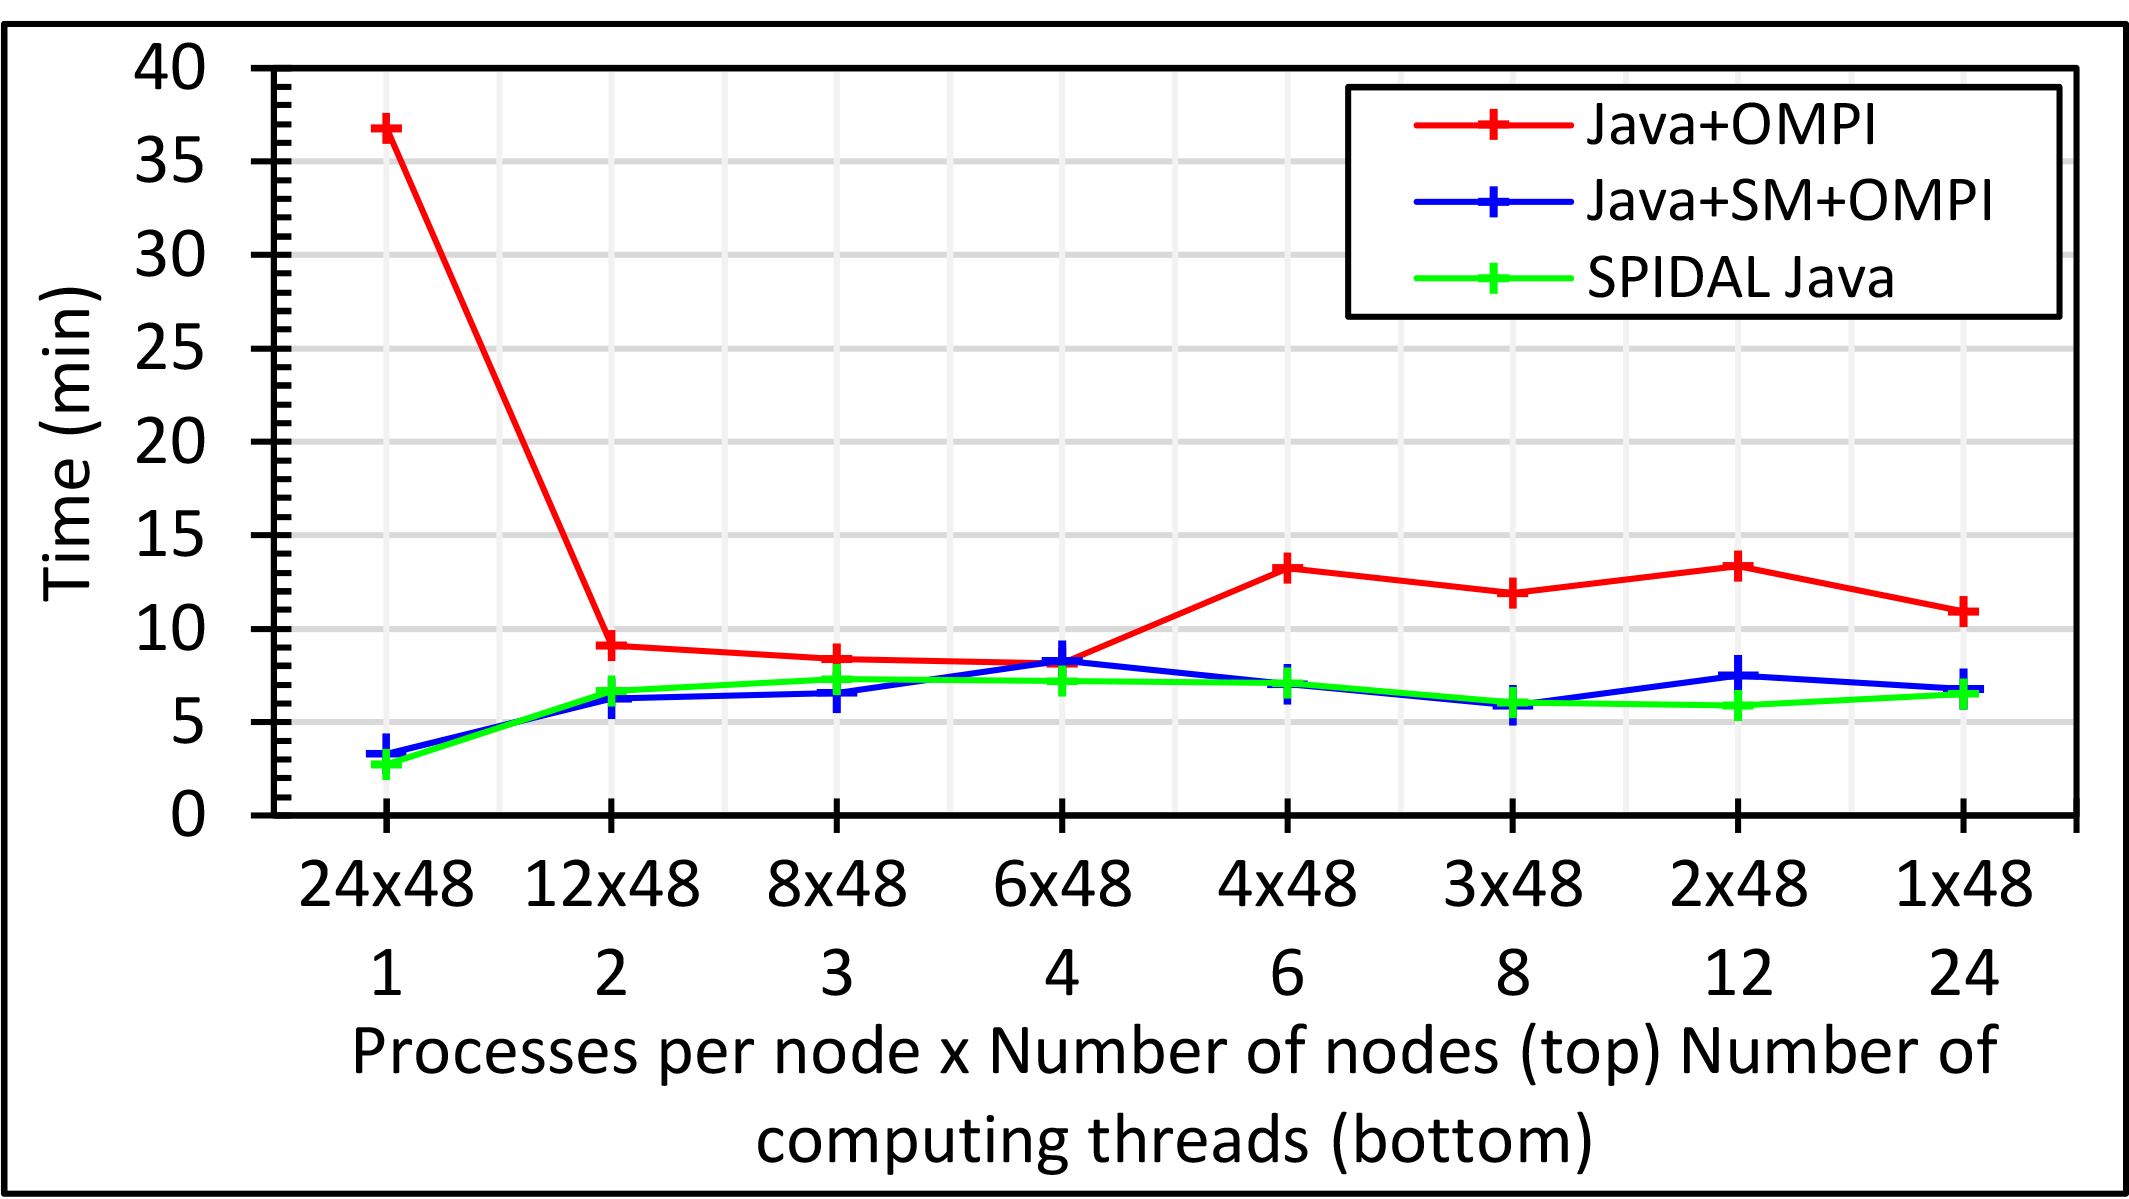
\includegraphics[width=0.85\columnwidth]{figures/fig_100K_TP}
        \caption{DA-MDS 100K performance with varying intra-node parallelism}
        \label{fig:fig_100K_TP}
    \end{minipage}%
    \begin{minipage}{0.49\textwidth}
        \centering
        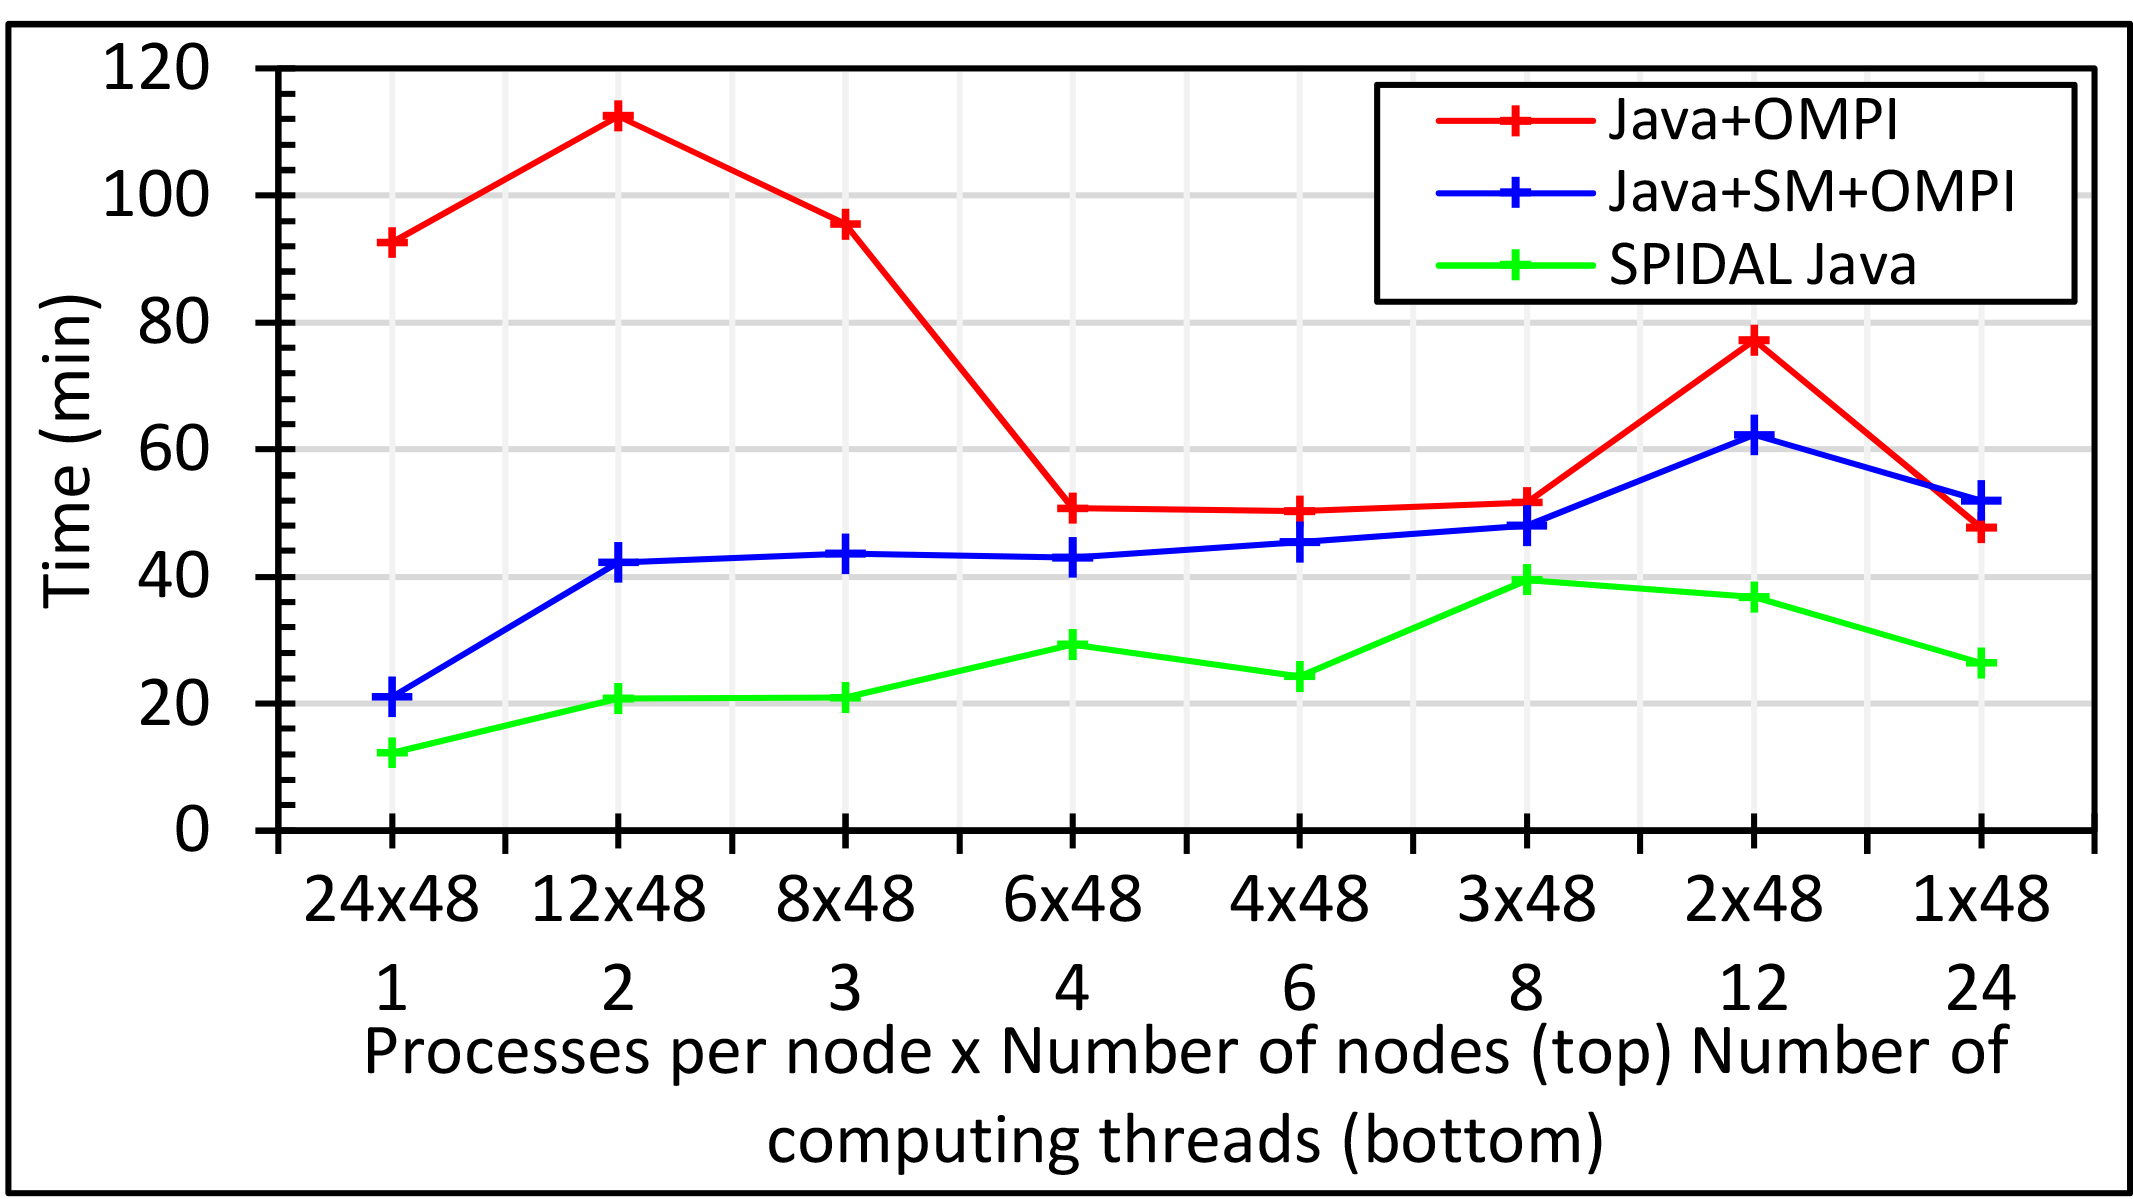
\includegraphics[width=0.85\columnwidth]{figures/fig_200K_TP}
        \caption{DA-MDS 200K performance with varying intra-node parallelism}
        \label{fig:fig_200K_TP}
    \end{minipage} 
    \begin{minipage}{0.49\textwidth}
        \centering
        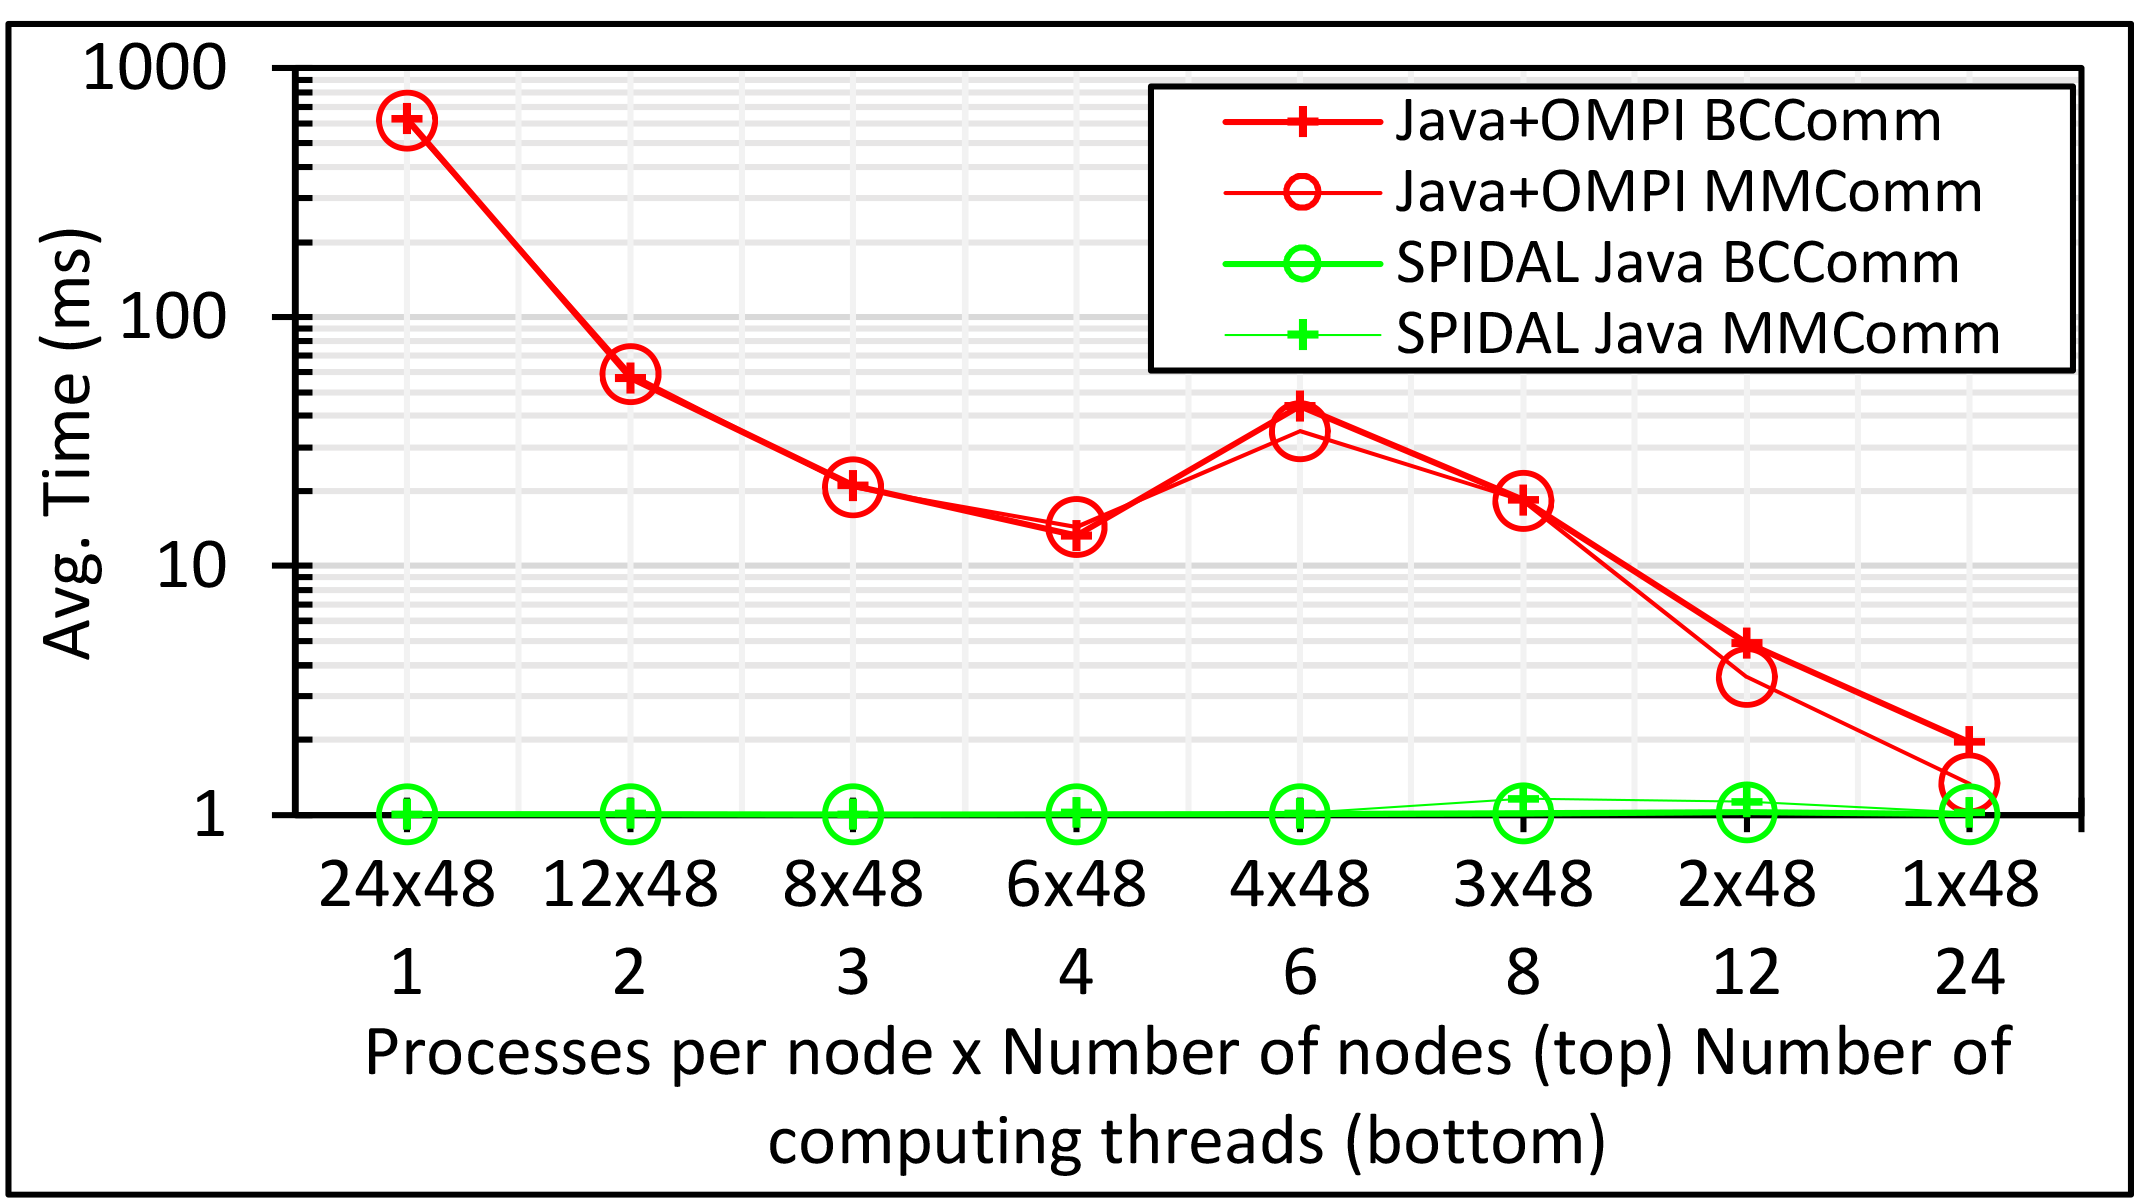
\includegraphics[width=0.85\columnwidth]{figures/fig_100K_TP_allgatherv}
		\caption{DA-MDS 100K \texttt{allgatherv} performance with varying intra-node parallelism}
        \label{fig:fig_100K_TP_allgatherv}
    \end{minipage}
    \begin{minipage}{0.49\textwidth}
        \centering
        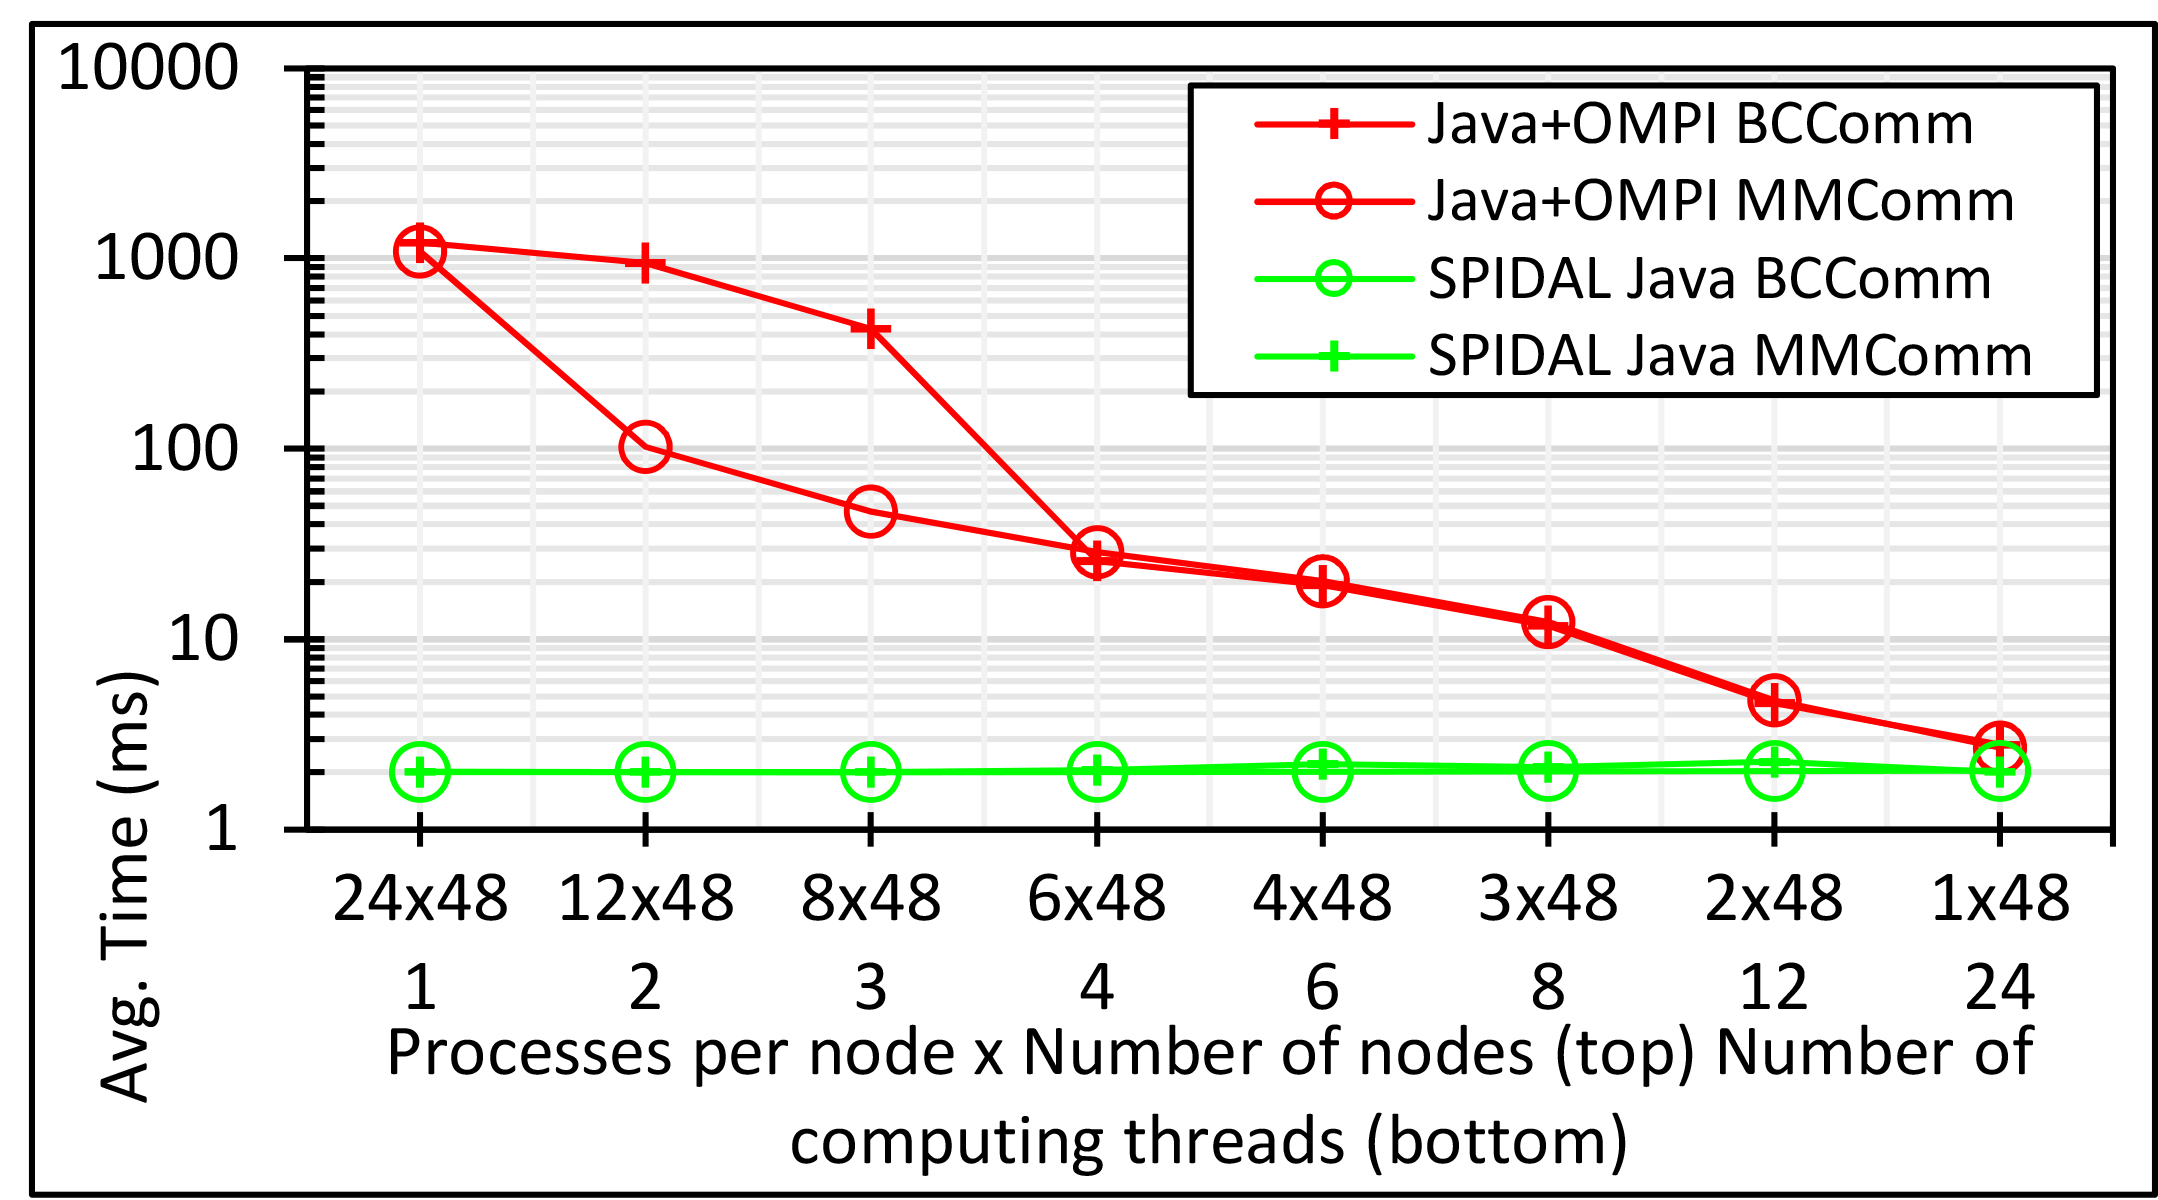
\includegraphics[width=0.85\columnwidth]{figures/fig_200K_TP_allgatherv}
		\caption{DA-MDS 200K \texttt{allgatherv} performance with varying intra-node parallelism}
		\label{fig:fig_200K_TP_allgatherv}
    \end{minipage}        
\end{figure*}     

\begin{figure*}[!htb]   
	\centering 
	\begin{minipage}{0.49\textwidth}
        \centering
        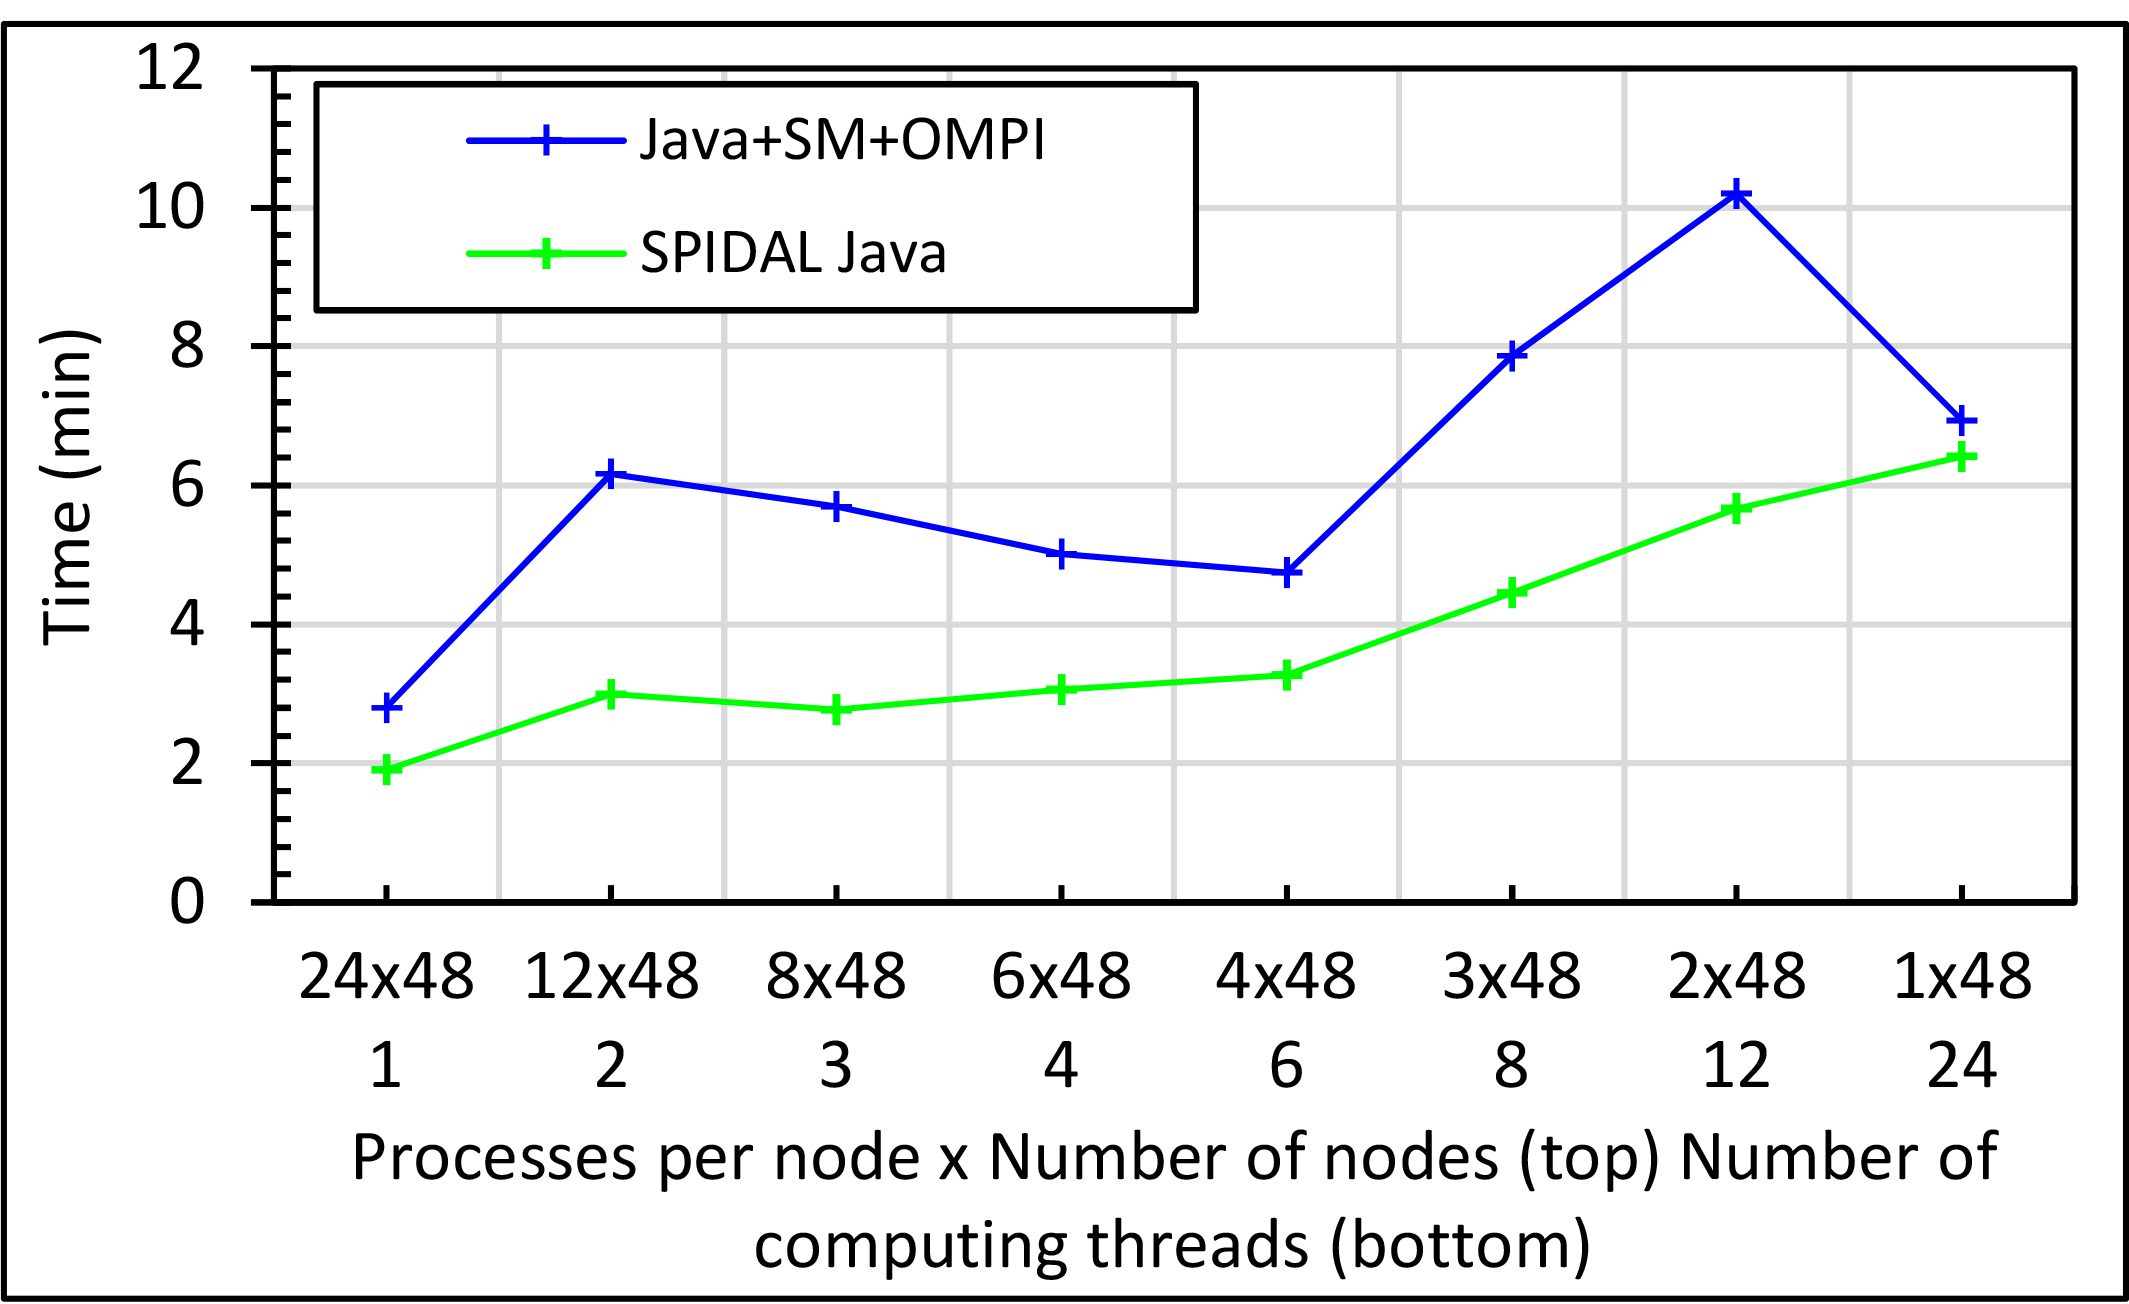
\includegraphics[width=0.85\columnwidth]{figures/fig_400K_TP}
        \caption{DA-MDS 400K performance with varying intra-node parallelism}
        \label{fig:fig_400K_TP}
    \end{minipage}
    \begin{minipage}{0.49\textwidth}
        \centering
        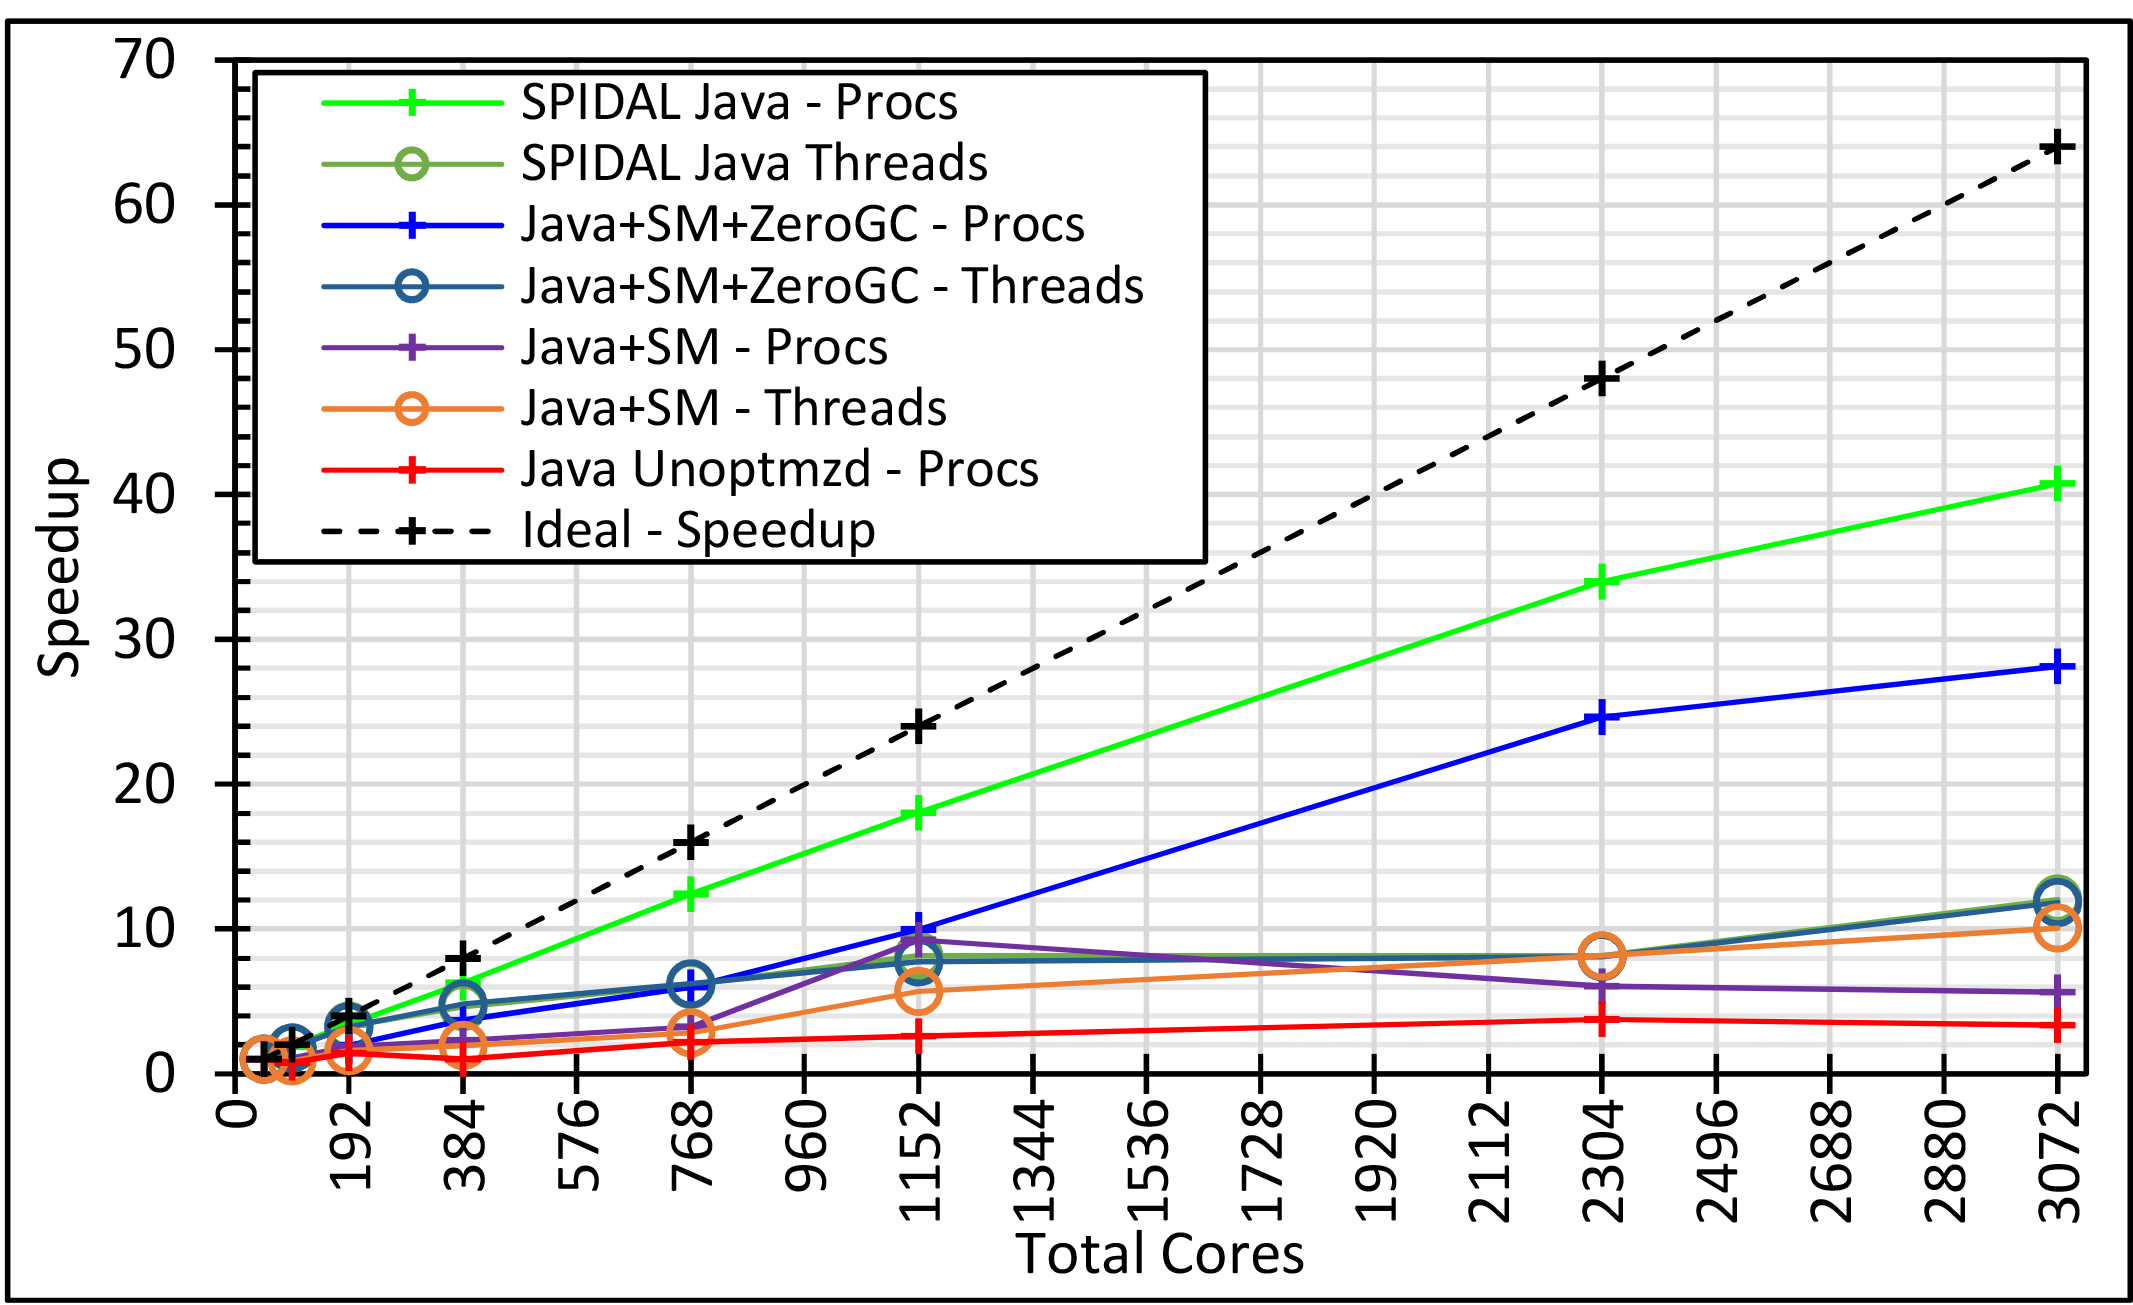
\includegraphics[width=0.85\columnwidth]{figures/fig_speedup_with_opts}
		\caption{DA-MDS speedup for 200K with different optimization techniques}
		\label{fig:fig_speedup_with_opts}
    \end{minipage}            
\end{figure*}

\begin{figure*}[!htb]   
	\centering 
    \begin{minipage}{0.49\textwidth}
        \centering
        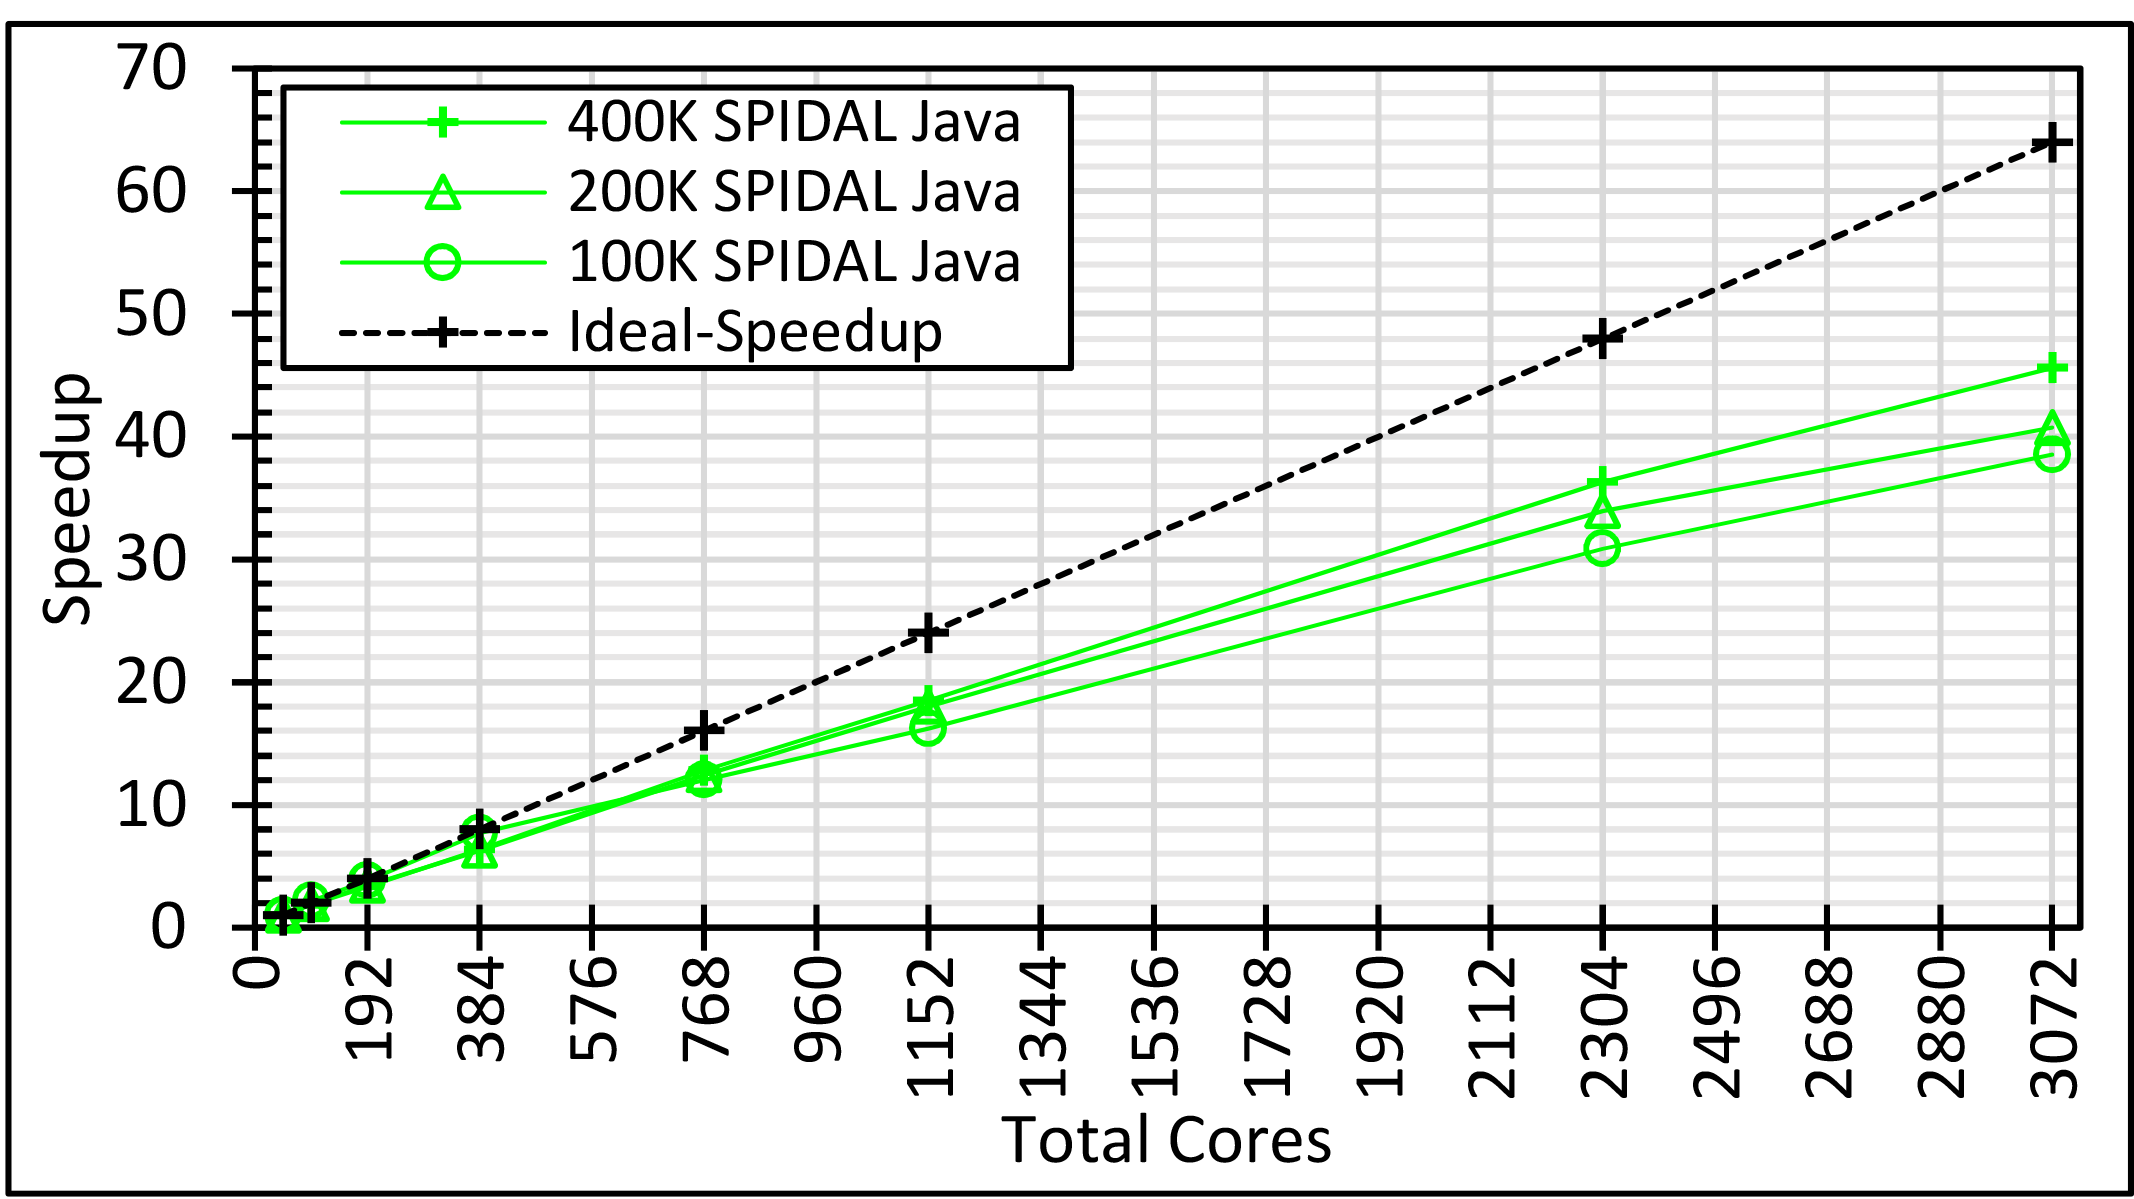
\includegraphics[width=0.85\columnwidth]{figures/fig_speedup}
		\caption{DA-MDS speedup with varying data sizes}
		\label{fig:fig_seepdup}
    \end{minipage}
    \begin{minipage}{0.49\textwidth}
        \centering
        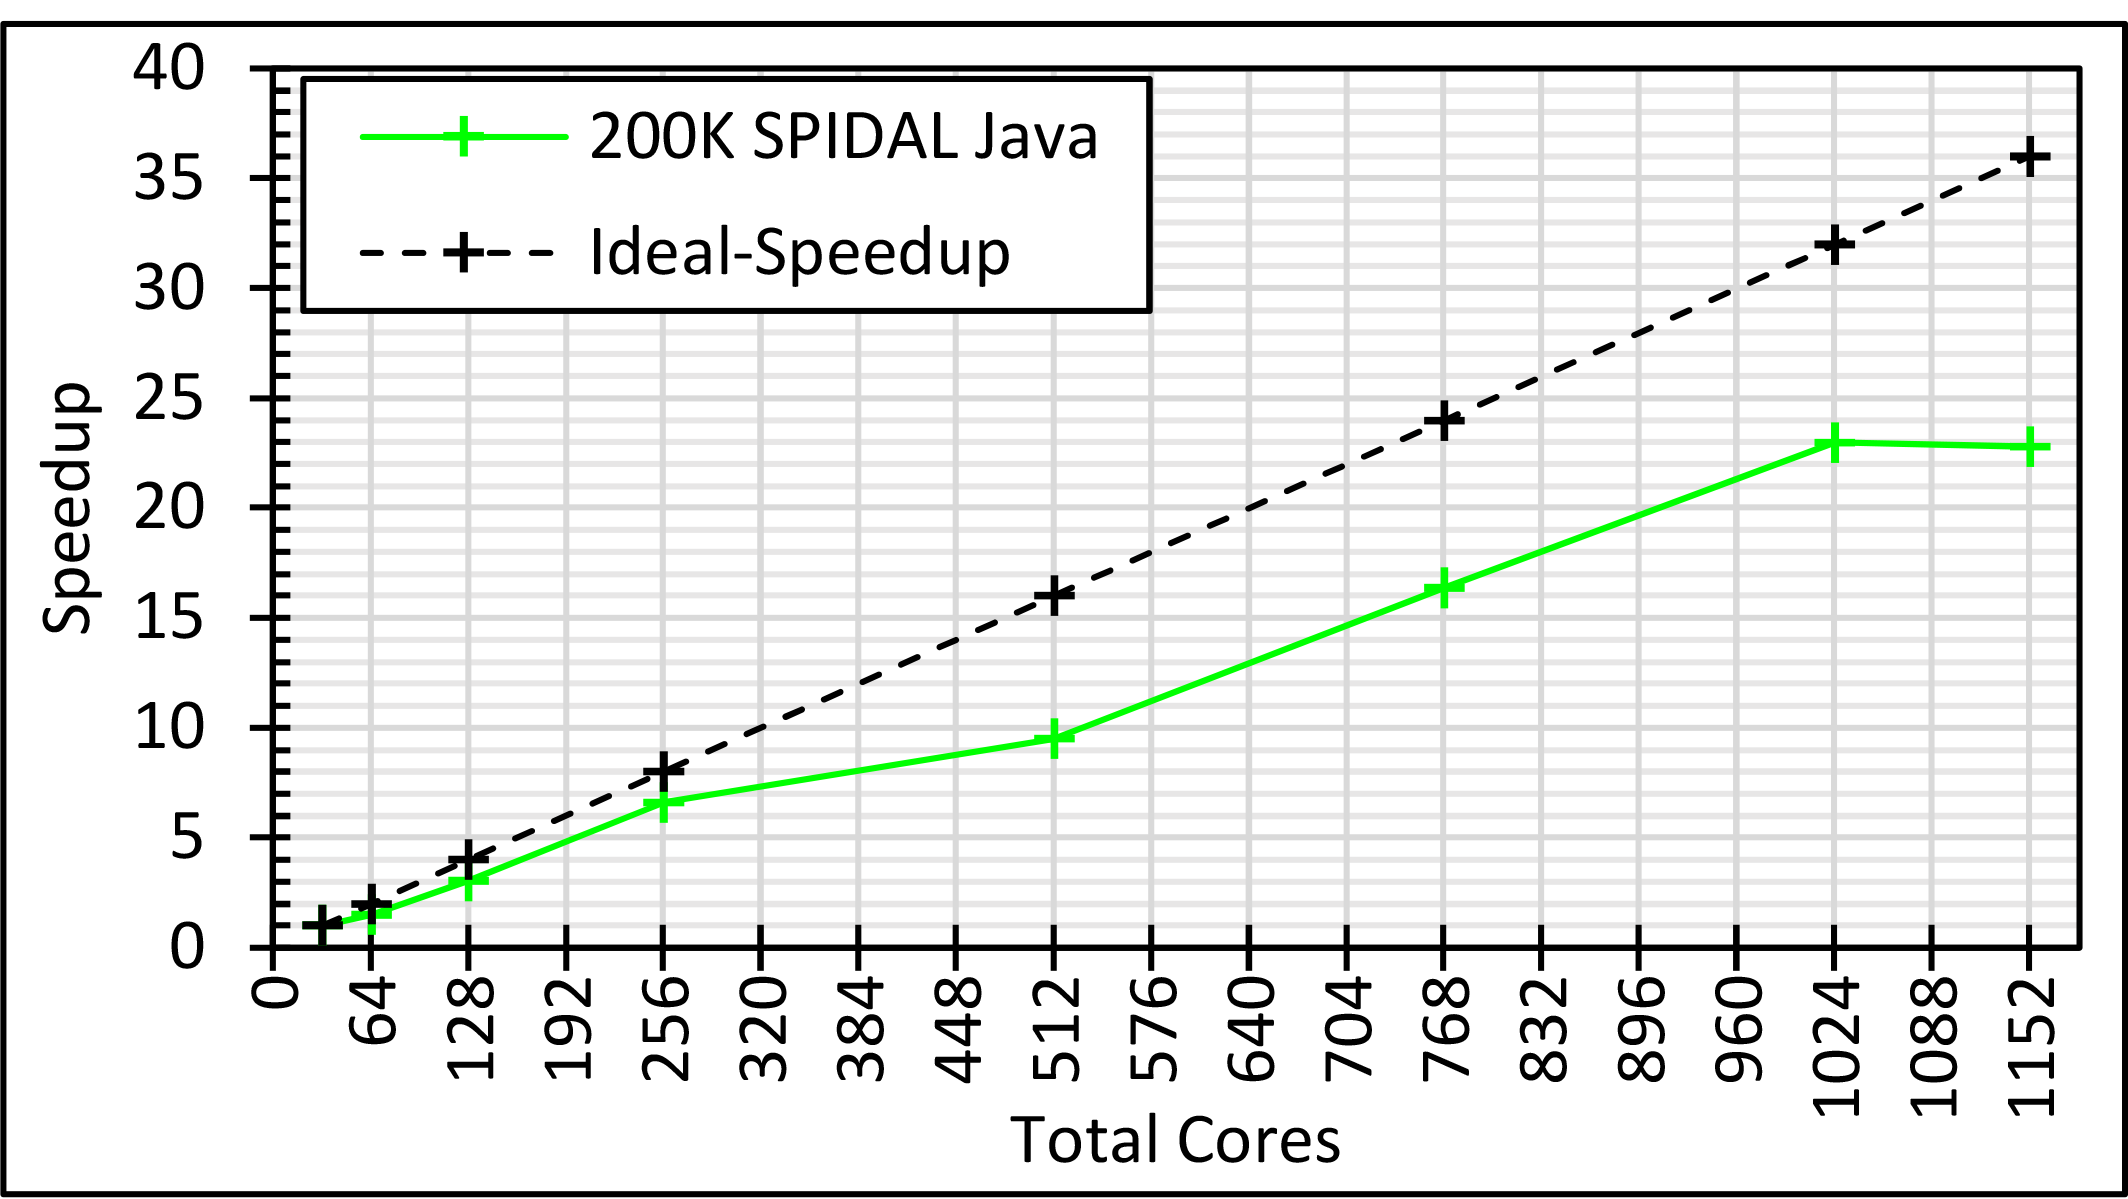
\includegraphics[width=0.85\columnwidth]{figures/fig_speedup_36core}
		\caption{DA-MDS speedup on 36 core nodes for 200K data}
		\label{fig:fig_seepdup_36core}
    \end{minipage}    
\end{figure*}

Patterns on the X-axis of the graphs show the combination of threads ($T$), processes ($P$), and the number of nodes. The total number of cores per node was 24 (12 on each socket), so the Figure \ref{fig:fig_100K_TP} through \ref{fig:fig_200K_TP_allgatherv} show all possible combinations that give 24-way parallelism per node. OpenMPI has a number of \texttt{allgather} implementations and these were using the linear ring implementation of MPI \texttt{allgatherv} as it gave the best performance. The Bruck \cite{Bruck:1997:EAA:271425.271434} algorithm, which is an efficient algorithm for all-to-all communications, performed similarly but was slightly slower than the linear ring for these tests.

Ideally, all these patterns should perform the same because the data size per experiment is constant, however, results show the default Java and OpenMPI based implementation significantly degrades in performance with large process counts per node (red-line). In addition, increasing the number of threads, while showing a reduction in the communication cost (Figure \ref{fig:fig_100K_TP_allgatherv} and \ref{fig:fig_200K_TP_allgatherv}), does not improve performance. The Java and OpenMPI memory mapped implementation (blue-line) surpasses default MPI by a factor of 11x and 7x for 100K and 200K tests respectively for all process (leftmost 24x48) cases. Cache optimization further improves performance significantly across all patterns especially with large data, as can be seen from the blue line to the green line (SPIDAL Java).

The DA-MDS implementation in SPIDAL Java, for example, has two call sites to MPI \texttt{allgatherv} collective, BCComm and MMComm, written using OpenMPI Java binding \cite{Vega-Gisbert:2013:TAJ:2488551.2488599}. They both communicate an identical number of data elements, except one routine is called more times than the other. Figures \ref{fig:fig_100K_TP_allgatherv} and \ref{fig:fig_200K_TP_allgatherv} show the average times in log scale for both of these calls during the 100K and 200K runs. 

SPIDAL Java achieves a flat communication cost across different patterns with its shared memory-based intra-node messaging in contrast to the drastic variation in default OpenMPI. Also, the improved communication is now predictable and acts as a linear function of total points (roughly 1ms to 2ms when data size increased from 100K to 200K). This was expected and is due to the number of communicating processes being constant and 1 per node.

Figure \ref{fig:fig_seepdup} shows speedup for varying core counts for three data sizes - 100K, 200K, and 400K. These were run as all processes because threads did not result in good performance. None of the three data sizes were small enough to have a serial base case, so the graphs use the 48 core as the base, which was run as 1x48 - 1 process per node times 48 nodes. SPIDAL Java computations grow $O(N^2)$ while communications grow $O(N)$, which intuitively suggests larger data sizes should yield better speedup than smaller ones and the results confirm this behavior. 

Figure \ref{fig:fig_seepdup_36core} shows similar speedup results when run on Juliet's 36 core nodes. The number of cores used within a node is equal to the X-axis' value divided by 32 - the total 36 core node count. It shows a plateau in speedup after 32 processes per node, which is due to hitting the memory bandwidth. 

Figure \ref{fig:fig_speedup_with_opts} shows DA-MDS speedup with different optimization techniques for 200K data. Also, for each optimization, it shows the speedup of all threads vs. all processes within a node. The total cores used range from 48 to 3072, where SPIDAL Java's 48 core performance was taken as the base case (green line) for all other implementations. The bottom red line is the Java and OpenMPI default implementation with no optimizations. Java shared memory intra-node messaging, zero GC, and cache optimizations were added on top of it. Results show that Java and OpenMPI with the first two optimizations (blue line) and all processes within a node surpass all other thread variations. This is further improved with cache optimization (SPIDAL Java - green line) and gives the best overall performance.

\todo{NAS table}

Table \ref{tab:table1} and \ref{tab:table2} show native Fortran and C performance against Java for a couple of NAS \cite{nas} serial benchmarks and block matrix multiplication in DA-MDS. Note. the native NAS implementations are directly obtained from the NAS benchmark site. Table \ref{tab:table1} also shows default NAS Java performance. Note, the 1x1 serial pattern in Table \ref{tab:table2} mimics the matrix sizes for 1 process in 24x48. The results suggest Java yields competitive performance using the optimizations discussed in this paper.